% Greedy half of the report. Uses the same preamble as sec_dc.tex.
% Figures are read from greedy/ because report.tex lives in the repository root.

\section{Greedy: Fewest Price Refreshes Under a Request Budget}
\label{sec:greedy}

\subsection{Problem}
\label{sec:greedy-problem}

Fare trackers learn of price changes only by querying the seller's site, as
in early airfare-prediction work~\cite{etzioni2003buy}, and a site may refuse
requests that arrive too fast~\cite{rfc6585}.
Cruise Finder~\cite{cruisefinder} is a self-hosted web application, written
by the second author, that tracks Carnival Cruise Line sailings from Florida.
It reads prices from Carnival's public but undocumented search endpoint,
calling it once per configured departure month and following every result
page. Because the endpoint is unofficial and rate-limited, the application
calls it only on demand and logs every call in an append-only audit table.
We call one pass over every configured month and every page a \emph{refresh
batch}; it observes the current price of every listed sailing. We assume
every batch costs the same, so the objective counts batches, not HTTP
requests (the number of pages can change over time).

We propose a feature that the application does not have today: \emph{quote
requests}. A quote request names a sailing and a window of days during which
one fresh observation of its price is acceptable. The question is: given every
request's window, what is the fewest refresh batches that give every window at
least one observation, and on which days?

For the case study we generate one request per sailing by a stated policy, a
modeling choice rather than a claim about how fares move. Each window opens at
Carnival's final-payment deadline, $76$ days before departure for cruises of
up to $5$ days and $91$ days for $6$ days or more~\cite{carnival481}, and
closes when booking closes, $c$ days before departure. Final payment is when
every booking must be paid in full; unpaid bookings are cancelled and their
cabins return to sale, so it is a natural moment to want a current quote. We
found no Carnival page giving the booking cutoff, so $c=2$ is an assumption.
The model asks for one observation per window, not continuous tracking, so it
minimizes refresh batches, not missed discounts or the average staleness that
crawler refresh policies optimize~\cite{cho2003refresh}.

\subsection{Abstraction}
\label{sec:greedy-abstraction}

Days are integers. Sailing $i$ departs on day $d_i$ and lasts $L_i$ days;
its window is $W_i=[a_i,b_i]$ with
\begin{equation}
a_i=d_i-F(L_i),\quad b_i=d_i-c,\quad
F(L)=\begin{cases}76 & L\le5,\\ 91 & L\ge6.\end{cases}
\label{eq:greedy-window}
\end{equation}
We take $L_i$ from the search data's duration field, which equals arrival
minus departure in days for every sailing we fetched and matches the
``$L$-Day'' length the table in~\cite{carnival481} uses. Windows with $b_i$ before
today are dropped, and $a_i$ is raised to today if it is earlier. A batch on
day $t$ observes every window with $t\in W_i$.

The abstract problem: given a set $\mathcal{W}=\{W_1,\dots,W_n\}$ of integer
intervals with $a_i\le b_i$, find a set of days $T\subseteq\mathbb{Z}$ that
\emph{hits} every interval ($T\cap W_i\ne\emptyset$ for all $i$) with $|T|$
minimum. This is the minimum point cover of intervals, also called interval
stabbing, equivalent to a minimum clique cover of the interval
graph~\cite{gupta1982interval}. It is not interval scheduling, which picks a largest set of pairwise
disjoint intervals; here we pick points that meet every interval.

\subsection{Algorithm}
\label{sec:greedy-algorithm}

\textsc{Refresh-Days} (Fig.~\ref{fig:greedy-alg}) scans the windows by
closing day. Whenever a window holds no chosen day yet, it chooses that
window's last day, the latest day that still serves it. The windows that
cause a choice are the \emph{witnesses}. On the windows $[1,10]$, $[4,12]$,
$[8,20]$, $[15,25]$, $[22,30]$ it chooses days $10$ and $25$ with witnesses
$[1,10]$ and $[15,25]$. One day cannot suffice, since $[1,10]$ and $[22,30]$
share no day.

\begin{figure}[t]
\begin{algorithmic}[1]
\STATE \textbf{function} \textsc{Refresh-Days}$(\mathcal{W})$
\STATE sort $\mathcal{W}$ so that $b_1\le b_2\le\dots\le b_n$
\STATE $T\gets\emptyset$;\ $S\gets\emptyset$;\ $\mathit{last}\gets-\infty$
\FOR{$i=1$ \TO $n$}
  \IF{$a_i>\mathit{last}$}
    \STATE $T\gets T\cup\{b_i\}$;\ $S\gets S\cup\{W_i\}$
      \COMMENT{greedy choice}
    \STATE $\mathit{last}\gets b_i$
  \ENDIF
\ENDFOR
\RETURN $T$, $S$ \COMMENT{refresh days, witnesses}
\end{algorithmic}
\caption{Fewest days hitting every window. $S$ is used only in the proof.}
\label{fig:greedy-alg}
\end{figure}

\subsection{Correctness}
\label{sec:greedy-correctness}

The proof follows the structural-bound pattern for greedy
algorithms~\cite{kleinberg2006algorithm}: the algorithm's choices exhibit
$m$ windows that force any solution to use $m$ days. Throughout, windows are
indexed in sorted order, and $\mathit{last}$ is the most recently added day,
so $\mathit{last}=\max T$ at every step.

\begin{lemma}[every window is covered]\label{lem:greedy-cover}
When \textsc{Refresh-Days} returns, every $W_i$ contains a day of $T$.
\end{lemma}
\begin{IEEEproof}
Consider the step that processes $W_i$. If $a_i>\mathit{last}$, line~6 adds
$b_i\in W_i$ to $T$. Otherwise $\mathit{last}\ne-\infty$, so
$\mathit{last}=b_j$ for some earlier $j<i$, and $b_j\le b_i$ by the sort.
Then $a_i\le b_j\le b_i$, so $b_j\in T$ lies in $W_i$. Days are never removed
from $T$.
\end{IEEEproof}

\begin{lemma}[witnesses are disjoint]\label{lem:greedy-disjoint}
The witnesses are pairwise disjoint, and $|S|=|T|$.
\end{lemma}
\begin{IEEEproof}
Each addition puts one window in $S$ and one day in $T$, and the days added
are strictly increasing ($b_i\ge\mathit{last}$ and $b_i\ge a_i>\mathit{last}$),
so $|S|=|T|$. Let $i_1<\dots<i_m$ be the indices that triggered additions,
and take $r<s$. When $i_s$ is processed, $\mathit{last}=b_{i_{s-1}}\ge
b_{i_r}$, because $\mathit{last}$ only increases and the $b$'s are sorted.
The test on line~5 passed, so $a_{i_s}>\mathit{last}\ge b_{i_r}$. Every day
of $W_{i_s}$ is at least $a_{i_s}$ and every day of $W_{i_r}$ is at most
$b_{i_r}$, so the two windows share no day.
\end{IEEEproof}

\begin{theorem}[optimality]\label{thm:greedy-opt}
$T$ hits every window, and every set $T'$ that hits every window has
$|T'|\ge|T|$.
\end{theorem}
\begin{IEEEproof}
Feasibility is Lemma~\ref{lem:greedy-cover}. Let $T'$ hit every window. It
contains a day in each of the $m=|S|$ witnesses, and since the witnesses are
pairwise disjoint (Lemma~\ref{lem:greedy-disjoint}), no day lies in two of
them. These $m$ days are therefore distinct, so $|T'|\ge m=|T|$.
\end{IEEEproof}

The same argument shows that $S$ is a largest set of pairwise disjoint
windows, since any $k$ disjoint windows need $k$ distinct days of $T$. That
the two numbers are equal is a known property of interval
graphs~\cite{golumbic2004algorithmic}.

Lemmas~\ref{lem:greedy-cover} and~\ref{lem:greedy-disjoint} and
Theorem~\ref{thm:greedy-opt} are machine-checked in Lean~4~\cite{lean4}
(Appendix~\ref{app:greedy-lean}), under the following correspondence:
\begin{center}\small
\begin{tabular}{@{}ll@{}}
Lemma~\ref{lem:greedy-cover} & \texttt{refresh\_covers}\\
Lemma~\ref{lem:greedy-disjoint} & \texttt{witnesses\_pairwise\_disjoint}\\
Theorem~\ref{thm:greedy-opt} & \texttt{refresh\_optimal}
\end{tabular}
\end{center}
The Lean \texttt{refresh} is the loop of Fig.~\ref{fig:greedy-alg} on a list
already sorted by closing day, carrying $\mathit{last}$ as an argument; the
sort itself, the window construction~\eqref{eq:greedy-window} and
Theorem~\ref{thm:greedy-time} are not formalized. The Lean proof of
Lemma~\ref{lem:greedy-disjoint} does not need the sort: each witness opens
after the previous one closes in any input order.

\subsection{Running Time}
\label{sec:greedy-analysis}

\begin{theorem}[running time]\label{thm:greedy-time}
\textsc{Refresh-Days} runs in $O(n\log n)$ time with a comparison sort and
uses $O(n)$ extra space. If the windows arrive sorted by closing day, it runs
in $O(n)$ time.
\end{theorem}
\begin{IEEEproof}
Line~2 is a comparison sort, $O(n\log n)$ time and $O(n)$ space for the
sorted copy. The loop runs $n$ times, and each iteration does one comparison
and at most two constant-time insertions (appending to lists, as days arrive
in increasing order). $T$ and $S$ hold at most $n$ items each. Without
line~2, only the $O(n)$ loop remains.
\end{IEEEproof}

Theorem~\ref{thm:greedy-time} is an upper bound. The sort is the only
superlinear step, so the measured time should grow like $n\log n$ unless the
input is pre-sorted.

\subsection{In the Language of the Problem}
\label{sec:greedy-domain}

Among the sailings not yet observed, look at the one whose quote window
closes soonest and refresh on its last open day. That batch also observes
every other sailing whose window is open that day; cross them off and repeat.
No schedule with fewer batches exists, because the sailings we refreshed
\emph{for} have windows that never overlap, so each one needed a batch of its
own. For the $383$ Carnival sailings from Miami, Port Canaveral, Tampa and
Jacksonville departing November 2026 through April 2027 (fetched October 26,
2026), three batches suffice: on October 30, 2026, January 14, 2027 and
March 30, 2027, over a $184$-day horizon (Fig.~\ref{fig:greedy-windows}).
Each sailing is observed once within its window, not nightly, so this is
three calls of the full search instead of one per day.

\subsection{Experiments}
\label{sec:greedy-experiments}

\begin{figure*}[!t]
\centering
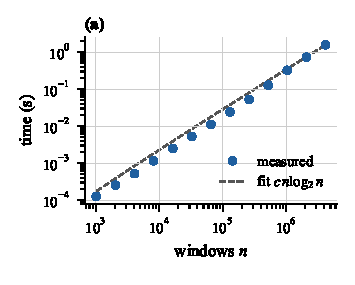
\includegraphics{greedy/figures/scaling}\hfill
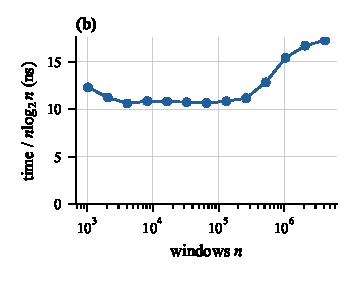
\includegraphics{greedy/figures/ratio}\hfill
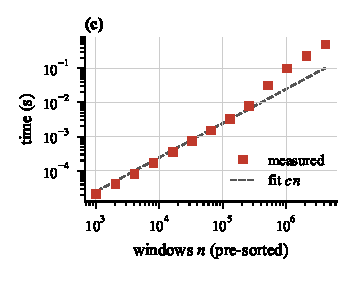
\includegraphics{greedy/figures/scan}
\caption{\textsc{Refresh-Days} on random windows. (a)~Running time with the
least-squares fit $c\,n\log_2 n$. (b)~Running time divided by
$n\log_2 n$; a flat curve confirms the growth rate. (c)~The scan alone on
pre-sorted windows, with the fit $c\,n$ over $n\le2^{17}$.}
\label{fig:greedy-scaling}
\end{figure*}

\begin{figure}[!t]
\centering
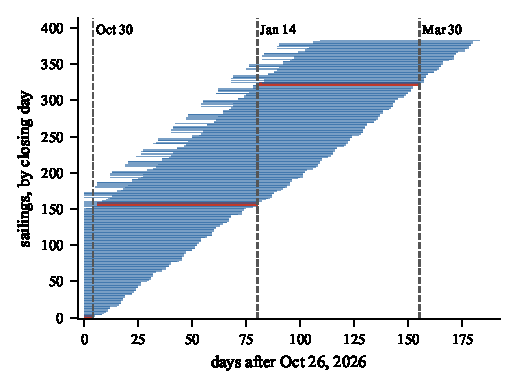
\includegraphics[width=\columnwidth]{greedy/figures/windows}
\caption{Quote windows of the $383$ real sailings, sorted by closing day.
Dashed lines are the three refresh days; the three witnesses are drawn
thick and red.}
\label{fig:greedy-windows}
\end{figure}

\textbf{Setup.} \textsc{Refresh-Days} was implemented in Python~3.12.2
(Appendix~\ref{app:greedy-code}) using the built-in sort, Timsort with the
powersort merge policy since Python~3.11~\cite{munro2018nearly}, and run on an AMD
Ryzen~7 9800X3D, following the protocol of Section~\ref{sec:dc-experiments}.
For $n=2^{10},\dots,2^{22}$ windows, departure days were drawn uniformly over
a horizon of $2n$ days, so that closing days are mostly distinct; a fixed
two-year horizon would make most windows tie. Cruise lengths were drawn from
the $383$ real sailings and windows built by~\eqref{eq:greedy-window} with
$c=2$. Each size was run five times on fresh inputs; we report the fastest
run with garbage collection disabled, as \texttt{timeit}
does~\cite{python-timeit}. Every run was checked to hit every window
(Lemma~\ref{lem:greedy-cover}) with one disjoint witness per day
(Lemma~\ref{lem:greedy-disjoint}). We also timed the scan alone on windows
already sorted by closing day. Unit tests additionally compare the output
with brute-force search on $300$ random instances of up to $10$ windows; this
checks the implementation on small cases, in the style of property-based
testing~\cite{claessen2000quickcheck}, and is not part of the proof.

\textbf{Running time.} Fig.~\ref{fig:greedy-scaling}(a) shows the time
following $c\,n\log_2 n$ over a $4096\times$ range of $n$, from
$0.1$\,ms to $1.6$\,s. In Fig.~\ref{fig:greedy-scaling}(b) the ratio is flat,
between $10.6$ and $12.3$\,ns, up to $n=2^{18}$, then rises to $17.3$\,ns at
$n=2^{22}$. The scan alone (Fig.~\ref{fig:greedy-scaling}(c)) costs
$20$ to $25$\,ns per window up to $n=2^{17}$, then up to $117$\,ns at
$n=2^{22}$. Both rises start around where the input, a list of Python tuples, no
longer fits in the processor's cache, and they are consistent with cache
misses~\cite{drepper2007memory}: after sorting, consecutive windows lie far apart in memory. Copying
the sorted windows into freshly allocated tuples cut the scan at $n=2^{22}$
from $118$ to $70$\,ns per window. The output size grew linearly, one refresh
day per about $39$ windows. Within the cache, the measurements match
Theorem~\ref{thm:greedy-time}: $n\log n$ with the sort, linear without it.
